\documentclass[a4paper,11pt]{article}


\usepackage{geometry}
\usepackage[utf8]{inputenc}
\usepackage[francais]{babel}
\usepackage[T1]{fontenc}
\usepackage{tikz-uml}
\usepackage{color}
\definecolor{dkgreen}{rgb}{0,0.6,0}
\definecolor{gray}{rgb}{0.5,0.5,0.5}
\definecolor{mauve}{rgb}{0.58,0,0.82}
\usepackage{listings}

\lstset{
language=C++,
basicstyle=\footnotesize,
backgroundcolor=\color{white},
keywordstyle=\color{red},
commentstyle=\color{dkgreen},
stringstyle=\color{mauve}, 
numberstyle=\color{red},
morekeywords={string},
frame=BL,
aboveskip=1em,
belowskip=2em,
}
\lstset{
  literate={ù}{{\`u}}1
           {é}{{\'e}}1
           {è}{{\'e}}1
           {à}{{\`a}}1
}


\lstdefinelanguage{tikzuml}{language=[LaTeX]TeX, classoffset=0, morekeywords={umlbasiccomponent, umlprovidedinterface, umlrequiredinterface, umldelegateconnector, umlassemblyconnector, umlVHVassemblyconnector, umlHVHassemblyconnector, umlnote, umlusecase, umlactor, umlinherit, umlassoc, umlVHextend, umlinclude, umlstateinitial, umlbasicstate, umltrans, umlstatefinal, umlVHtrans, umlHVtrans, umldatabase, umlmulti, umlobject, umlfpart, umlcreatecall, umlclass, umlvirt, umlunicompo, umlimport, umlaggreg}, classoffset=1, morekeywords={umlcomponent, umlsystem, umlstate, umlseqdiag, umlcall, umlcallself, umlfragment, umlpackage}, classoffset=0,  sensitive=true, morecomment=[l]{\%}}

\geometry{margin=2cm}
\geometry{headheight=15pt}

\usepackage{fancyhdr}
\usepackage{fancyvrb} 
\usepackage{graphicx}
\usepackage{float}

\pagestyle{fancy}
\rhead{PFA - GuitarTutor}


\begin{document}

\begin{titlepage}
  \begin{center}

    \textsc{\LARGE PFA - GuitarTutor}\\[2cm]
    Pacien \textsc{Boisson} \ \ \ Jean-Michaël \textsc{Célerier}  \ \ \ Julien \textsc{Chaumont}\\
    Abdelhamid \textsc{Cherif} \ \ \ Alban \textsc{De Martin} \ \ \ Kun \textsc{Jiao} \ \ \ Bastien \textsc{Meunier} \\[3cm]
    \textsc{\large 29/03/2013 }\\[1.5cm]
    
\includegraphics[width=8cm]{logo.png}

  \end{center}
  \vspace{3cm}
  \begin{flushleft}
   \underline{Clients :} Pierre \textsc{Hanna}, Matthias \textsc{Robine}\\
   \underline{Responsable pédagogique :} Julien \textsc{Allali}
  \end{flushleft}


\end{titlepage}

\clearpage

\section*{Introduction}
%Dans cette partie, j'ai repris quasiment mot pour mot l'intro que j'avais écrite pour le cahier des charges.

\subsection*{Serious game}

En quelques années, les jeux vidéos ont su attirer un public immense et éclectique. Alors qu'ils étaient réservés, il y a encore quelques années, à un public bien ciblé, les éditeurs ont su s'ouvrir à toute une gamme de joueurs jusqu'alors insoupçonnés - l'appellation casual gamer était née. Aujourd'hui, les recherches dans le domaine vidéo-ludique vont encore plus loin. A l'aide de technologies toujours plus poussées, toujours plus proches du joueur et de son environnement, il est désormais possible d'interagir avec lui, grâce à ses mouvements par exemple. Et pourquoi pas par le son? Les jeux de rythme, remontant pourtant aux bornes d'arcade des années 1990, ont connu un immense succès avec la sortie de jeux tels que Guitar Hero en 2005, qui a ouvert la voie à de nombreux remakes que sont Just Dance ou encore Band Hero. En parallèle, les jeux à caractère éducatifs, ont été pendant longtemps recalés au rang de “sous-jeux” de par leurs gameplays souvent repoussants et des graphismes généralement peu soignés - 
évidemment, les budgets ne sont pas forcément les mêmes.

Le projet GuitarTutor se place au croisement de ces deux genres pour s'inscrire dans celui très fermé des serious games: pourquoi ne pas apprendre en s'amusant? (En l'occurrence l'apprentissage de la guitare). Ce jeu s'adresse à des élèves d'écoles de musique débutant la pratique de l'instrument. L'objectif est de les encourager à jouer et à s'entraîner en dehors des heures de cours avec leurs professeurs, en faisant intervenir cet univers ludique, pour les inciter à persévérer et à travailler d'eux-mêmes.

\subsection*{Le logiciel avant le PFA}

Le logiciel GuitarTutor reposait sur des travaux de recherches du LABRI, ainsi que sur le travail fourni par des élèves de l'ENSEIRB-MATMECA dans le cadre des Projets au Fil de l'Année (PFA) de 2011-2012. La base du projet consistait en l'analyse d'accords en temps réel, c'est-à-dire pouvoir donner précisément le nom de l'accord qui est donné en entrée audio de l'ordinateur. La librairie EHPCP a donc été codée à cet effet. En complément, le développement d'une interface graphique, à l'aide de la librairie Qt, a été réalisée. Celle-ci assurait le fonctionnement basique d'un logiciel permettant de visualiser une liste défilante d'accords ainsi que le résultat de la partie analyse de l'entrée audio, en comparant cette donnée au résultat attendu.

Afin de faciliter l'écriture de ces fichiers partitions, un second logiciel avait été mis en place à destination du professeur. Il permettait une édition totalement manuelle de grilles d'accords, ainsi qu'une édition assistée. Ce second mode d'édition demandait à l'utilisateur de marquer les accords d'un morceau joué simultanément par l'appui sur une touche de son clavier. Dans un deuxième temps, il suffisait d'indiquer quels étaient les accords qui correspondaient à chaque pulsation.

\subsection*{Notre objectif}

L'objectif de notre projet était donc de rendre le logiciel existant accessible. Son interface d'origine avait, en effet, plus la carrure d'un prototype que celle d'un produit fini. Un soin particulier devait être apporté à l'éditeur de partitions afin d'optimiser au mieux l'expérience utilisateur. Selon les demandes clients, GuitarTutor devait être un logiciel fini et livrable pour avril 2013.

\clearpage

\tableofcontents

\clearpage

\section{Architecture logicielle}

Nous présenterons dans cette partie la structure du projet actuel, ainsi que celle de sa version d'origine.

\subsection{Architecture du projet d'origine}

\subsection{Le modèle MVC}

Le modèle MVC, pour \textit{Modèle, Vue, Contrôleur}, constitue une architecture logicielle particulière qui se base sur la différenciation de deux parties dans un programme:
\begin{itemize}
 \item Les données (le modèle)
 \item L'interface graphique (la vue)
\end{itemize}
Le contrôleur se place entre ces deux entités, en agissant comme relais en synchronisant les informations qui transitent de l'une à l'autre.

L'avantage immédiat du modèle MVC est l'organisation du code qu'il induit, ainsi que la facilitation de la maintenance de celui-ci.

\subsection{Editeur, Lecteur et API}

Il nous a été conseillé dès le début du projet d'adopter le modèle MVC. En plus des avantages cités précédemment, cela nous permettait de découvrir le code existant, de mieux le comprendre, et de commencer à le réorganiser correctement. L'architecture qui a été retenue était de découper le projet en trois parties:
\begin{itemize}
 \item L'interface graphique du lecteur
 \item L'interface graphique de l'éditeur
 \item Le reste: l'API
\end{itemize}
L'idée était de mettre ce \textit{reste} dans une bibliothèque qui serait appelée à la fois par l'éditeur et par le lecteur (même si ce ne sont pas forcément les mêmes parties qui les intéressent). La figure \ref{mvc} résume cette organisation.

\begin{figure}[!ht]
\begin{center}
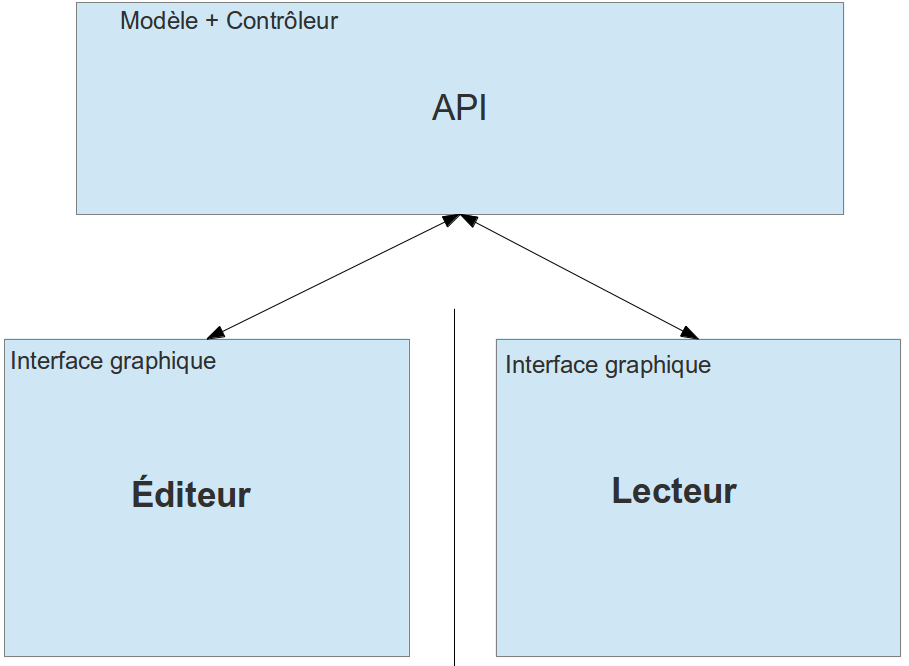
\includegraphics[width=450px]{mvc.png}
\caption{Le modèle MVC dans notre code}
\label{mvc}
\end{center}
\end{figure}

\subsection{Diagramme de classes}

\subsection{Quelques points particuliers}

\clearpage

\section{Problèmes rencontrés, problèmes résolus}

Le développement de GuitarTutor ne s'est pas fait sans heurts. Nous sommes néanmoins parvenus à résoudre les différents problèmes auxquels nous avons été confrontés.

\subsection{Reprise de code}

Comme c'était prévu, la reprise du code existant fut notre première grande étape de développement. Passé le moment de découragement lié à l'absence total de commentaires et de documentation dans la grande majorité du code source qui nous intéressait, nous nous sommes attelés à ``débroussailler'' le dépôt en mettant en place une documentation, en commentant le code, ainsi qu'en supprimant purement et simplement les portions inutilisées, qui représentaient tout de même une portion loin d'être négligeable (parfois de simples fonctions, parfois des fichiers, et parfois des dossiers entiers\dots).

Passés ces quelques semaines de nettoyage et d'assimilation du code existant, nous avons pu apporter les modifications qui était demandées.

\subsection{Refonte de l'interface du lecteur}

\subsection{Portabilité}

La portabilité du logiciel, notamment sur Mac OS et Windows, faisait partie des principales demandes des clients. Les librairies utilisées jusque là était censées fonctionner à la fois sur Mac OS, Windows et GNU/Linux, et c'était une bonne raison pour ne pas en changer.

Nous nous sommes cependant rapidement rendus à l'évidence: on ne développe pas un logiciel portable simplement en utilisant des librairies portables.

\subsubsection*{Sur Mac OS}

Personne, dans notre équipe, n'ayant une machine sous Mac OS, nous avons dû nous contenter d'une version de Mountain Lion en machine virtuelle. Outre un problème d'extrême lenteur lors de la compilation et divers autres soucis liés à la connexion internet et la reconnaissance des ports USB, il était impossible de vérifier le bon fonctionnement du lecteur, puisque l'entrée audio de la VM n'était pas activé. Nous avons donc pendant longtemps développé \textit{``à l'aveugle''} sous Mac OS, où tout ce que nous pouvions faire était de vérifier que la compilation se faisait correctement.

Fort heureusement, un test sur une vraie machine Mac début mars nous a confirmé que le projet était bien compatible, et nous en avons également profité pour vérifier le fonctionnement de notre installateur.

\subsubsection*{Sur Windows}

%Qt5, l'installateur, boost,...

\subsubsection*{Sur GNU/Linux}

Il s'agit du seul des trois systèmes d'exploitation pour lequel nous n'avons pas eu de problème particulier, mais aussi le seul qui n'était pas demandé. Peut-être est-ce simplement parce que nous avons tous commencé à coder directement sur celui-ci.

\clearpage

\section{Discussion sur les choix opérés}

\subsection{Environnement logiciel}

Comme il nous avait été conseillé de faire, nous nous sommes rapidement accordés sur l'environnement logiciel a adopter.
\begin{itemize}
 \item Utilisation de QtCreator, environnement de développement C++ open-source, multi-OS, et régulièrement mis à jour
 \item Développement sur Linux. Le choix n'était pas évident, étant donné que cet OS n'était pas censé devoir être ciblé. L'intérêt était en fait de ne pas favoriser le développement sur Windows, avant de nous rendre compte que certains de nos choix avaient été faits au détriment de Mac OS, ou inversement.
 \item Utilisation du gestionnaire de version Git, et non de SVN. La raison est que Git est de plus en plus utilisé, au détriment de SVN, et que le PFA était une excellente occasion pour apprendre à l'utiliser.
 \item Création du dépôt sur GitHub. Nous avons éliminé le dépôt de l'ENSEIRB-MATMECA en raison d'une coupure qui aura duré plusieurs jours en octobre (en plus des fréquentes interruptions de ce service dont nous avions pris l'habitude au cours de l'année passée), ainsi que de nombreux autres services tels que Sourceforge ou Google Code, car ceux-ci imposaient l'utilisation d'une licence libre (ce qui, a priori, n'est pas le cas de GuitarTutor) aux projets hébergés sur leur plate-forme, à moins de payer un abonnement mensuel. GitHub était également dans ce cas, mais une offre réservée aux étudiants nous a permis de bénéficier gratuitement d'un compte premium pour créer librement un dépôt privé, sans contrainte de licence.
\end{itemize}


\subsection{Utilisation de Qt}

Le choix d'utiliser la librairie Qt s'est fait très rapidement, tant les avantages étaient évidents:
\begin{itemize}
 \item Le code source existant utilisait déjà Qt
 \item Qt est utilisable aussi bien sur Mac OS que sur Windows, ainsi que sur Linux
 \item Le développement avec Qt est facilité par l'IDE que nous avions choisi, à savoir QtCreator
 \item La documentation est très claire et complète
 \item Qt est open-source et bénéficie d'une large communauté d'utilisateurs
 \item Qt est incroyablement complet: interface graphique, XML, multimédia, socket,\dots
 \item Plusieurs d'entre nous avions déjà des connaissances sur cette librairie
\end{itemize}

Nous avons donc choisi d'adopter cette librairie dès les débuts du projet.

\subsection{Utilisation de FMOD}

FMOD est la librairie audio qui est utilisée aujourd'hui dans l'éditeur. Là encore, c'était cette même librairie qui servait déjà dans l'ancienne version de l'éditeur, dans la partie qui traitait les fichiers audio. Nous aurions pu faire le choix d'utiliser libsndfile, comme c'est le cas dans le lecteur, mais il faut reconnaître que l'éditeur n'a pas besoin d'une gestion aussi bas niveau du son. FMOD nous a donc semblé être un bon choix, malgré le fait qu'il s'agisse d'un code propriétaire (nous n'avons pas eu de contre-indication de la part des clients à ce propos).

\subsection{Format d'échange en XML}



\subsection{Reprise des bases précédentes}

Même s'il était au départ tentant de faire table rase et de recommencer le projet à zéro, tant la présentation du code existant laissait à désirer, nous avons fait l'effort de le remanier et de l'appréhender afin de pouvoir le réutiliser au maximum.

\subsubsection{Sur l'éditeur}

Nous avons gardé la base de l'interface de l'éditeur, à savoir le système de grilles, ainsi que le système d'arbre des accords. Nous avons ensuite ajouté peu à peu les différents éléments qui constituent aujourd'hui l'éditeur de grilles (voir figure \ref{av_ap_editeur}).

\begin{figure}[!ht]
\begin{center}
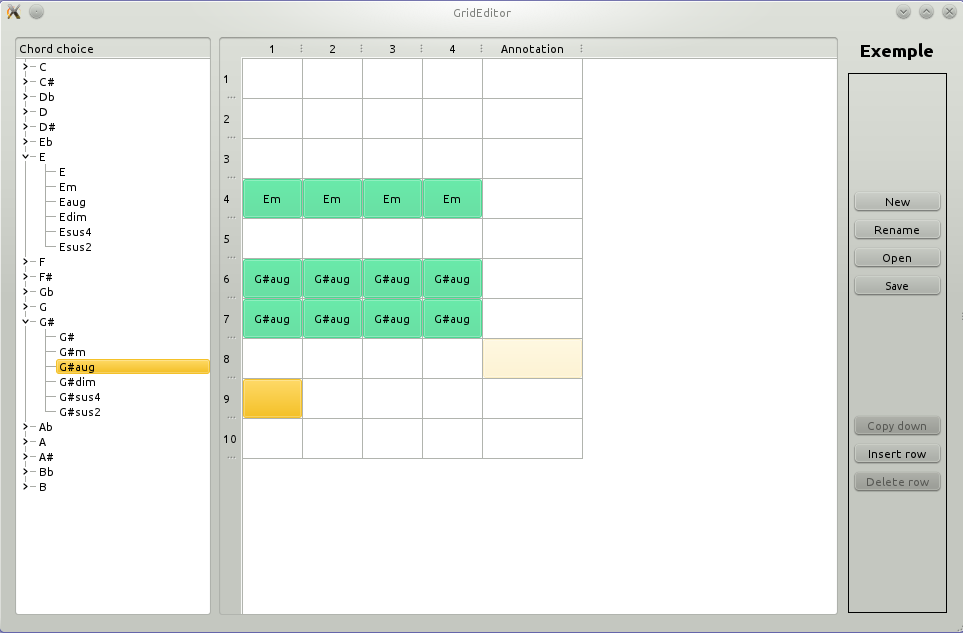
\includegraphics[width=225px]{ancien_editeur.png}
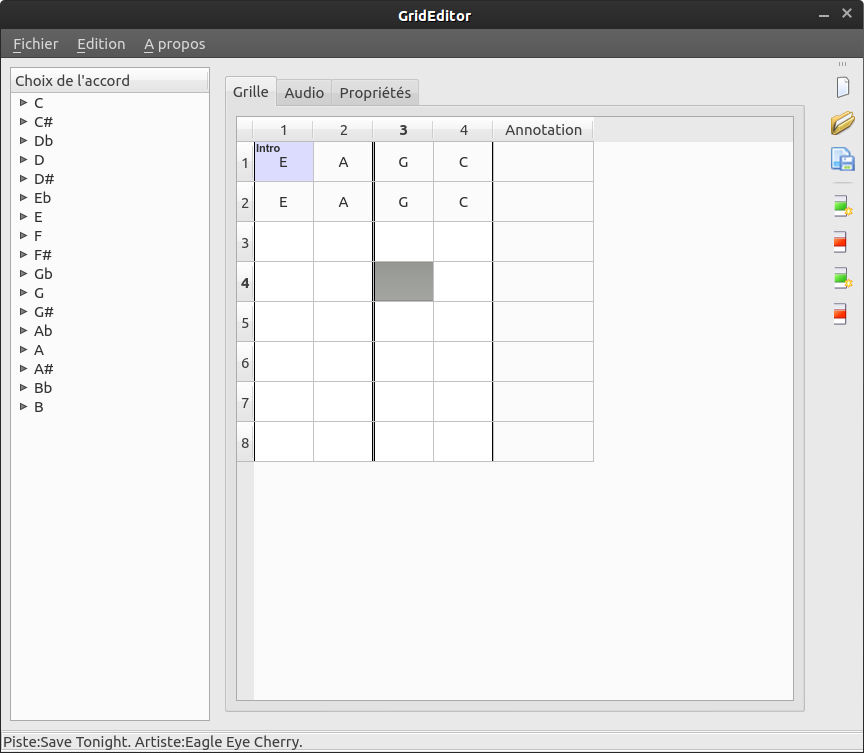
\includegraphics[width=225px]{nouveau_editeur.png}
\caption{L'éditeur de grilles, avant et après}
\label{av_ap_editeur}
\end{center}
\end{figure}

Nous avons fait le choix de penser en premier lieu à l'expérience utilisateur, en créant une interface qui soit à la fois accessible et esthétique. Nous avons par exemple apporté:
\begin{itemize}
 \item la traduction en Français de l'interface
 \item la possibilité d'ajouter les accords au clavier, comme il serait tentant de faire
 \item une meilleure visibilité du découpage en mesures et en parties de la grille
 \item une barre d'outils pour les actions les plus fréquentes, ainsi que des raccourcis claviers
 \item le rapprochement implicite entre la grille et le morceau (système d'onglets, et fusion des deux anciens éditeurs en un seul)
 \item \dots
\end{itemize}

\subsubsection{Sur le lecteur}

En ce qui concerne le lecteur, nous n'avons finalement changé que l'interface. La plupart des fichiers qui se trouvent aujourd'hui dans l'API, notamment \texttt{ScoreManager} et \texttt{MusicManager}, ainsi que la librairie \textit{IScoreLight}, n'a pas ou peu été retouchée. Comme indiqué précédemment, l'interface a, elle, été refaite à zéro.

\subsection{Installateurs sur les différents systèmes d'exploitation}

\subsection{Développement agile}

En accord avec les conseils de notre responsable pédagogique, nous avons rapidement opté pour l'utilisation d'une méthode de développement de type agile. Le PFA état en effet une excellente occasion pour s'essayer à ce genre de méthodes qui sont de plus en plus employées dans des cadres professionnels. 

\subsubsection{Réunions clients}

Dès le mois de novembre, nous avons mis en place un système de rendez-vous réguliers, généralement toutes les trois semaines avec nos clients. Ces réunions servaient tout d'abord à présenter le travail qui avait été effectué depuis le dernier rendez-vous, au travers d'une démonstration sur le logiciel en cours de développement. S'en suivait une discussion sur les différents points qui méritaient d'être relevés, afin de répartir les tâches en trois catégories: ce qui était fait et qui était validé, ce qui était fait mais restait à améliorer (ou à changer totalement), et enfin, ce qui restait à faire. Il ne restait alors qu'à fixer les objectifs à tenir d'ici le prochain rendez-vous.

Les avantages de travailler de la sorte se sont révélés au cours du projet. Tout d'abord, la possibilité de discuter de manière régulière de nos avancées avec nos clients était particulièrement intéressante, car cela permet d'instaurer un dialogue entre demandeurs et réalisateurs. On peut notamment remarquer que le cahier des charges (cf annexes) comporte plusieurs points qui n'ont pas été réalisés, ou qui ont été réalisés différemment de ce qui était initialement prévu, pas à cause d'un manque de temps, mais grâce à ce dialogue qui a permis d'affiner et de changer les besoins exprimés au fur et à mesure du développement du projet.

La figure \ref{agile} résume ce processus.

\begin{figure}[!ht]
\begin{center}
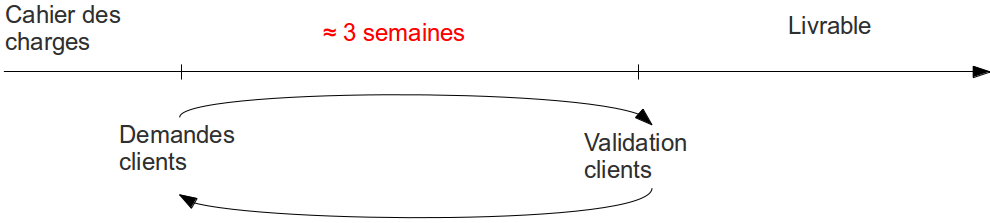
\includegraphics[width=450px]{methode_agile.png}
\caption{Schéma du processus de développement agile}
\label{agile}
\end{center}
\end{figure}

\subsubsection{Organisation de l'équipe et du travail}

De manière analogue au \textit{ScrumMaster} de la méthode Scrum, nous avons choisi au sein de notre équipe une personne en charge de veiller à la bonne application de notre méthode de développement. Sans se situer à un niveau supérieur aux autres, comme ce serait le cas pour un chef de projet, cette personne devait centraliser les travaux et les impressions de chacun pour aider à la répartition des tâches. Elle servait par ailleurs de \textit{représentant} de notre équipe pour nos clients et notre responsable pédagogique.

Les tâches étaient ensuite attribuées selon les demandes du cycle courant et des préférences de chacun, généralement par binômes. Des réunions hebdomadaires permettaient de faire le point sur les difficultés rencontrées et l'avancement des différentes tâches, et éventuellement de réorganiser la répartition. En plus de cela, l'équipe était informée par mail des interrogations et des avancées entre deux réunions, ainsi que par l'intermédiaire de notre wiki que nous avons mis en place dès le début du projet.

De manière générale, cette méthode de développement semble avoir bien fonctionné pour notre équipe au cours de ce projet.

\clearpage

\section*{Conclusion}
%Ce que nous a apporté le projet
%Apprentissage de librairies complexes
%Si chacun veut mettre un mot personnel ici...

\clearpage





















\begin{titlepage}
  \begin{center}
    \vspace{8cm}
    \Huge \textbf{Annexes}
  \end{center}
\end{titlepage}

\clearpage

\section*{Cahier des charges}\label{cdc}

\textit{Ce document rédigé par nos soins constitue le cahier des charges qui a été validé par nos clients début janvier 2013.}

\vspace{1cm}

Il a été souligné la nécessité de garder à l'esprit le public visé afin de le cibler au mieux - à savoir les professeurs de guitare d'une école de musique et leurs élèves, ainsi qu'une population de ``joueurs'' désirant s'initier ou s'améliorer à la guitare. L'interface et les fonctionnalités des logiciels du projet devront donc être adaptés en conséquence, en visant à la fois l'accessibilité et l'ergonomie. En outre, lors des entretiens avec les clients, de nombreux points ont été soulevés et soumis à notre évaluation. Nous les détaillerons dans cette partie.

\subsubsection*{Relatifs à l'ensemble du projet}

Les points suivants s'appliquent à l'ensemble du projet, c'est-à-dire à la fois à l'éditeur et au player.
\begin{itemize}
 \item \underline{Deux logiciels :} les parties éditeur et player devront être séparées en deux exécutables
 \begin{itemize}
  \item De cette façon, l'éditeur sera réservé au professeur.
  \item Le player sera quant à lui accessible au professeur et à son élève.
 \end{itemize}
 \item \underline{Mac OS X et Windows :} le projet devra pouvoir être utilisable intégralement sur ces deux systèmes d'exploitation.
 \begin{itemize}
  \item A cet effet, nous reprendrons les bibliothèques Qt, FMOD et Portaudio utilisées dans les précédentes versions du logiciel, et qui ont l'avantage d'être multi-OS.
  \item Le livrable sera fourni sous la forme d'un installateur pour chacun de ces OS.
 \end{itemize}
 \item \underline{Interface :} comme il a été souligné précédemment, un soin particulier sera attaché à l'interface utilisateur pour la rendre la plus intuitive et attrayante possible.
 \begin{itemize}
  \item Pour cela, nous créerons une version traduite en Français
  \item Des menus d'aide seront également présents pour accompagner les utilisateurs
 \end{itemize}
 \item \underline{Version finale :} le logiciel devra être fini et prêt au déploiement dans l'école de musique cliente pour avril 2013.
\end{itemize}

\subsubsection*{Relatifs à l'éditeur}

Les besoins propres à l'éditeur et nos propositions pour y répondre sont énumérés dans cette partie. L'éditeur permettra la saisie des accords d'un morceau par le professeur directement dans une grille.

L'éditeur est destiné à créer une grille d'accords sans assistance. Il se présente sous la forme d'une grille dont chaque case correspond à une mesure, et chaque ligne à une phrase.

\begin{itemize}
 \item \underline{Saisie :} la saisie des accords se fait soit case par case, soit en sélectionnant directement toutes les cases correspondant au même accord.
 \begin{itemize}
  \item Les accords se rentrent soit à la main, soit à l'aide d'un menu listant tous les accords reconnus par le logiciel.
  \item Afin de faciliter la saisie, les derniers accords utilisés seront mis en évidence.
  \item L'utilisateur pourra également indiquer la tonalité du morceau qu'il veut saisir pour que soient mis en évidence les accords les plus utilisés pour cette tonalité.
 \end{itemize}
 \item \underline{Écoute :} pour l'aider lors de la saisie, l'utilisateur pourra écouter directement via l'éditeur le fichier mp3 qu'il aura sélectionné.
 \begin{itemize}
  \item Les fonctionnalités les plus courantes d'un lecteur audio seront implémentées, telles que la pause, la reprise et le retour en arrière.
  \item Il est à noter que cette lecture audio ne servira qu'à l'utilisateur, pas au logiciel. Néanmoins, le chemin vers ce fichier sera retenu afin de pouvoir le réutiliser en changeant de mode d'édition, ou lors de la lecture par le Player de la partition créée.
 \end{itemize}
 \item \underline{Synchronisation audio :} pour que la partition créée soit utilisable par le Player, il faut qu'une information de tempo soit précisée par l'utilisateur.
 \begin{itemize}
  \item Pour cela, l'utilisateur sera invité à ouvrir le fichier mp3 correspondant à sa saisie (s'il ne l'a pas déjà fait pour s'aider lors de cette même saisie).
  \item Une fenêtre l'invitera à démarrer le fichier mp3 et à appuyer deux fois sur la touche espace de son clavier.
  \item Ces deux appuis délimiteront la durée d'une case de la grille.
  \item Si besoin est, il pourra recommencer cette étape à sa guise.
  \item Cette étape est facultative si l'utilisateur ne souhaite pas utiliser sa partition sur le player.
 \end{itemize}
\end{itemize}

\underline{Fonctionnalités générales de l'éditeur}

Afin que l'utilisateur puisse accéder à n'importe quel moment aux partitions qu'il aura créées, il se verra offrir la possibilité d'exporter sa grille d'accords dans un fichier.

\begin{itemize}
 \item \underline{Export :} deux formats de fichiers seront utilisables pour sauvegarder la partition sur le disque dur de l'utilisateur.
 \begin{itemize}
  \item Un premier format dit “grille” adoptera les conventions de l'école de musique cliente et servira pour impression.
  \item Un second format basé sur le langage xml permettra l'utilisation de la partition sur le player. L'étape de synchronisation audio devra être validée au préalable.
  \item Ces deux formats ne sont pas incompatibles, c'est-à-dire que la partition pourra être sauvegardée aussi bien dans un format que dans l'autre, et pourquoi pas dans les deux en même temps.
 \end{itemize}
 \item \underline{Import :} pour permettre d'éditer une partition dont la saisie a déjà été commencée, il sera possible de charger un fichier grille ou xml généré préalablement par l'éditeur. La grille d'accords sera remplie comme il se doit avec les données du fichier.
\end{itemize}

L'interface devra également permettre une plus grande flexibilité que l'actuelle au niveau des morceaux. Il devra par exemple être possible de modifier le nombre de cases par ligne en cours de saisie, ainsi que de générer des partitions aux mesures irrégulières. Dans ce cas, l'export au format grille serait autorisé, mais celui au format xml nécessitera au préalable que l'utilisateur indique tous les changements de mesures ainsi que les durées de chaque case dans ces portions.

\subsubsection*{Relatifs au player}

La partie jouable du projet est déjà fonctionnelle. Il faudra cependant veiller à y apporter quelques nouveautés.

\begin{itemize}
 \item \underline{Deux modes :} un mode orienté jeu et un mode orienté apprentissage
 \begin{itemize}
  \item Le mode jeu se basera sur un score calculé en deux étapes
  \begin{itemize}
   \item A-t-il joué le bon accord?
   \item L'a-t-il tenu assez longtemps?
  \end{itemize}
  \item Le mode apprentissage bouclera sur les différentes parties du morceau jusqu'à ce que le joueur les réussisse parfaitement.
 \end{itemize}
 \item \underline{Interface :} plus attrayante et plus ergonomique
 \begin{itemize}
  \item Proposer un mode plein écran
  \item Indiquer au joueur son avancée dans la partition au cours de la partie
  \item Mode horizontal ou vertical
 \end{itemize}
 \item \underline{Enchaînement :} possibilité de jouer plusieurs morceaux à la suite
 \item \underline{Entrées audio :} gestion des différentes entrées audio de l'ordinateur.
 \begin{itemize}
  \item Une extension intéressante serait de développer un mode multijoueur.
 \end{itemize}
\end{itemize}


\begin{figure}[!ht]
\begin{center}
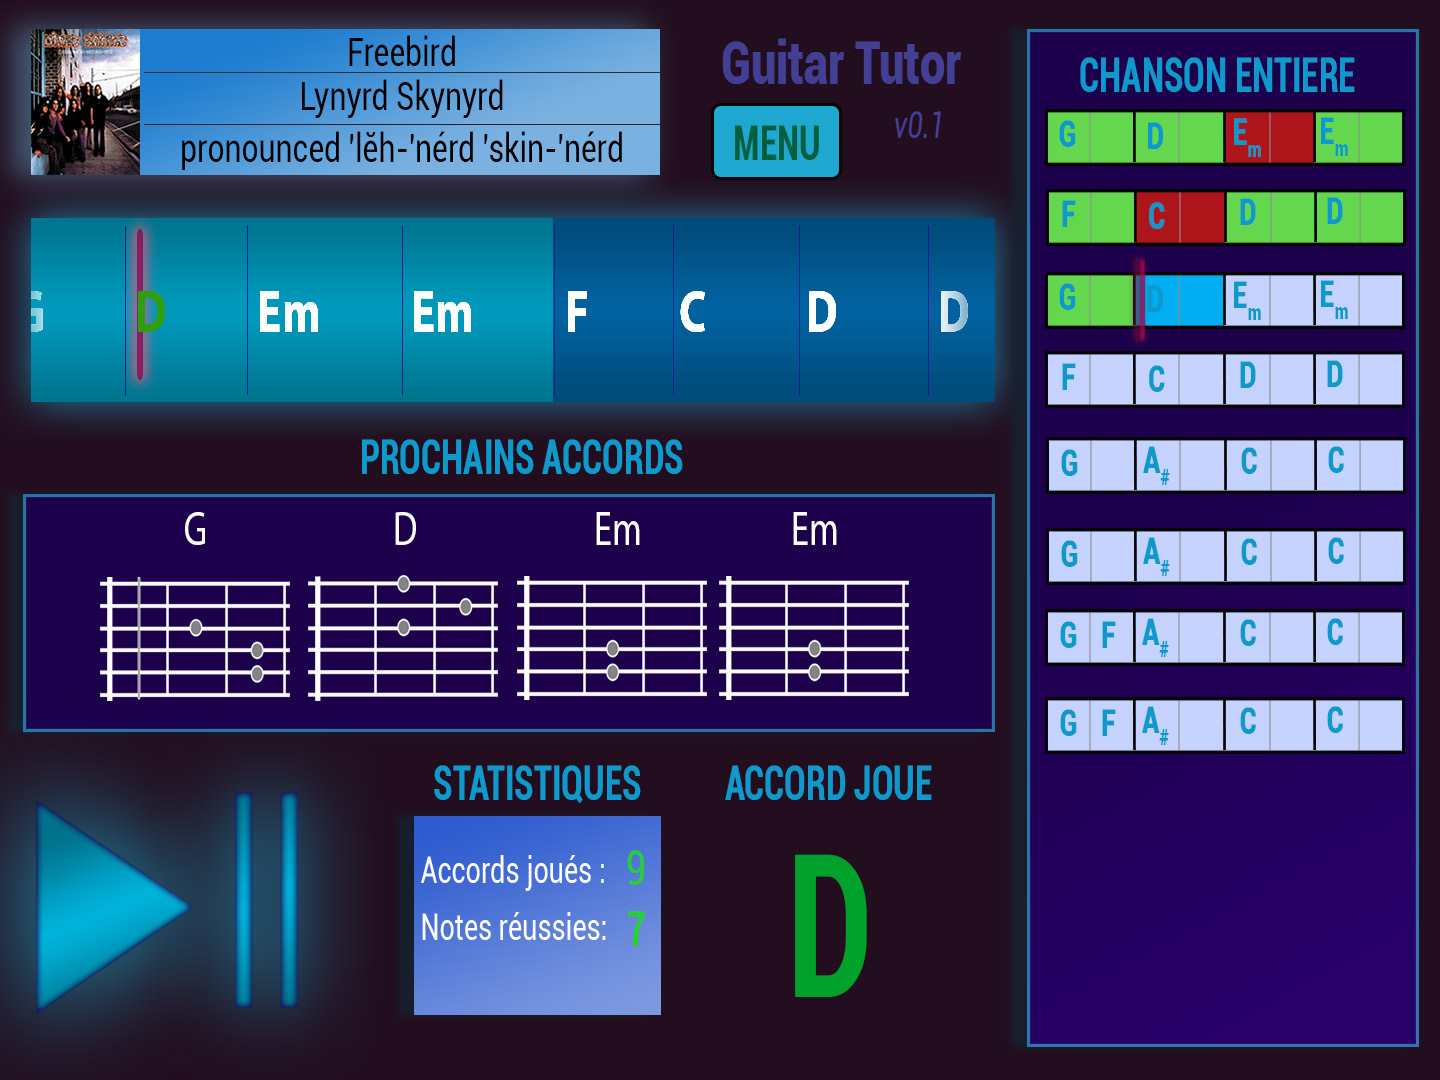
\includegraphics[width=450px]{interface_player_prototype.jpg}
\caption{Prototype d'interface pour le player}
\end{center}
\end{figure}


\subsubsection*{API GuitarTutor}

Afin de faciliter la maintenance du code source et l'extension des fonctionnalités, nous axerons nos premières étapes de développement sur la création d'une API commune à l'éditeur et au player dans le but de respecter une architecture Modèle Vue Contrôleur (MVC). Cette méthode de développement n'ayant pas été utilisée par nos prédécesseurs, il nous faudra un certain temps pour reconstruire proprement le projet, mais nous sommes certains que cela sera un gain de temps pour la suite du développement.

\clearpage

\end{document}
